\documentclass{article}
\usepackage[utf8]{inputenc}
\usepackage{tikz}

\title{flow}
\author{Iwo Gross}
\date{December 2022}
\usetikzlibrary{shapes.geometric, arrows, animations}

\tikzset{
  animate/shake/.style = {myself:xshift = { begin on=click,
      0s = "0mm", 50ms = "#1", 150ms = "-#1", 250ms = "#1", 300ms = "0mm" }}}
\tikzstyle{startstop} = [rectangle, rounded corners, text centered, draw=black,thick, minimum width=3cm, minimum height=1cm]
\tikzstyle{io} = [trapezium, trapezium left angle=70, right angle =110, text centered, minimum width=3cm, minimum height=1cm]
\tikzstyle{function} = [rectangle, text centered, draw=black,thick, minimum width=3cm, minimum height=1cm]
\tikzstyle{arrow} = [thick, ->, >=stealth]

\begin{document}
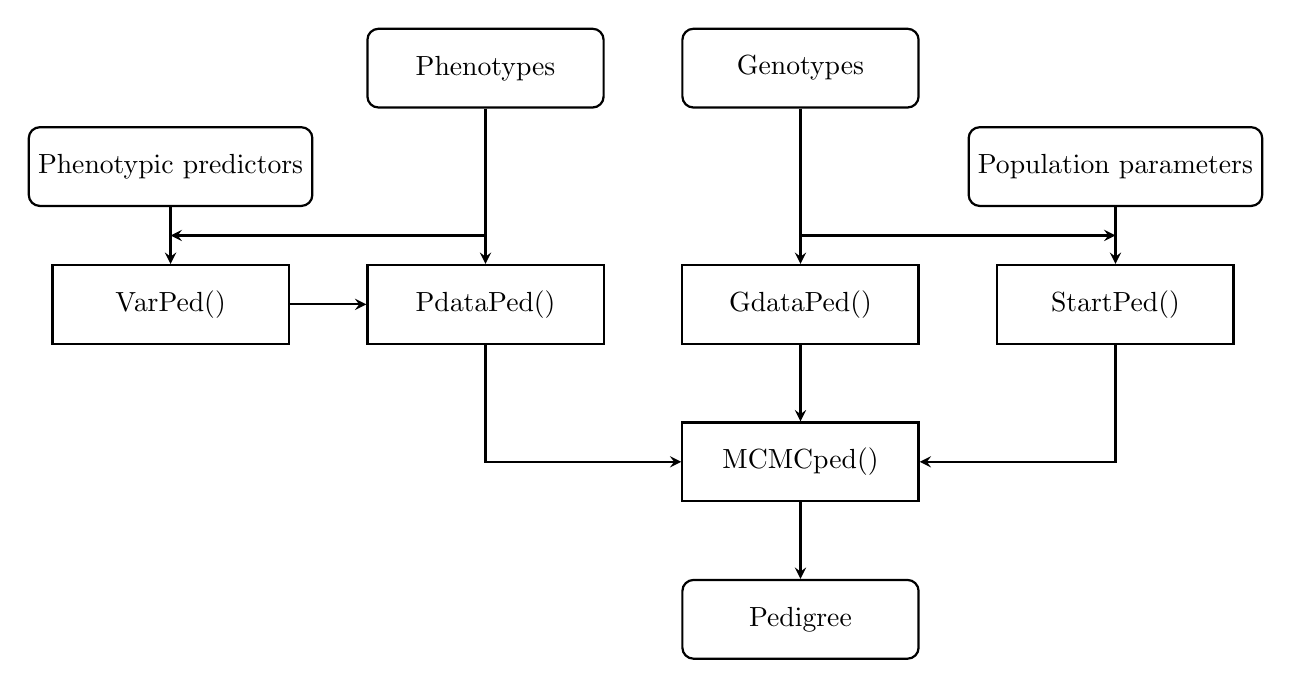
\begin{tikzpicture}[node distance=2cm]

\node (finalped) [startstop, animate = {shake = 2mm}] {Pedigree};
\node (mcmcped) [function, above of = finalped] {MCMCped()};
\node (gdataped) [function, above of = mcmcped] {GdataPed()};
\node (pdataped) [function, left of = gdataped, xshift=-2cm] {PdataPed()};
\node (startped) [function, right of = gdataped, xshift=2cm] {StartPed()};
\node (guppyg) [startstop, above of = gdataped, yshift=1cm] {Genotypes};
\node (varped) [function, left of = pdataped, xshift=-2cm] {VarPed()};
\node (preds) [startstop, above of = varped, yshift=-.25cm] {Phenotypic predictors};
\node (guppyp) [startstop, above of = pdataped, yshift=1cm] {Phenotypes};
\node (params) [startstop, above of = startped, yshift=-.25cm] {Population parameters};

\draw [arrow] (mcmcped) -- (finalped);
\draw [arrow] (gdataped) -- (mcmcped);
\draw [arrow] (pdataped) |- (mcmcped);
\draw [arrow] (startped) |- (mcmcped);
\draw [arrow] (guppyg) -- (gdataped);
\draw [arrow] (varped) -- (pdataped);
\draw [arrow] (preds) --coordinate[midway](m1)(varped);
\draw [arrow] (guppyp) -- (pdataped);
\draw [arrow] (guppyp) |- (m1);
\draw [arrow] (params) --coordinate[midway](m2)(startped);
\draw [arrow] (guppyg) |- (m2);

\end{tikzpicture}
\end{document}
